
\section{Discussion}
The period under study, July 1999 through to May 2001, showed no
clear seasonal wind signal with upwelling and downwelling winds
distributed year-around. Similar results were obtained by
\citet{Nogueira98}, who found that only 20\% the variability in
daily Ekman transport off Cape Finisterre over 9 years was
associated with the seasonal cycle, while 70\% concentrated at
frequencies $<$30 days.onal cycle, while 70\% was concentrated at
frequencies $<$30 days. \citet{Nogueira97} showed from harmonic
analysis that the average upwelling event length was $T=15\pm 5$
days, close to our estimate of $14\pm 2$ days. Comparing our data
with those of \citet{Kosro91} off California, we observe that
although cycles of upwelling-winds/relaxation take place in both
regions, Galicia is more variable in wind speed, direction and
persistence. Much of the summer variability relates to
anticyclones moving northeastward over the bay of Biscay.

Differing patterns of upwelling favourable wind fields force
different responses in the system favoring either north or west
coast upwelling (PUNC and PUWC, respectively). Summer 1999
experienced winds favorable to north coast upwelling and Cape
Finisterre filament development while summer 2000 was more
typified by west coast upwelling. Both years experienced highly
variable winds that did not persist long enough for upwelling
filaments to develop on the west coast. The strongest development
of west coast filaments in recent years occurred in 1998, when
west coast upwelling-favorable winds lasted from June to early
August with few interruptions. These sustained upwelling favorable
winds maintained a sharp upwelling front that allowed the
development and growth of the west coast instabilities into
upwelling filaments.

Much has been hypothesized about the generation of upwelling
filaments.  \citet{Roed99} and \citet{Haynes93} reported a clear
link between bottom topography and filament formation in the
Galician region on the basis of models and observations,
respectively. However, in the case presented here, the Cape
Finisterre filament is clearly dependent on particular wind
conditions for its development. The mere presence of upwelling at
Finisterre is not sufficient. Although small scale instabilities
sometimes develop off the Cape (see Figs~\ref{fig:windssst2123}b,d
and \ref{fig:windssst95}a), it requires a well developed north
coast upwelling for them to grow into a full sized filament. At
these times the wind field is like that of
Fig~\ref{fig:windsreconfig}a and the filament extends offshore
along the line of maximum wind curl identified in mode 2 in
Fig~\ref{fig:windseofseasonal}.
\begin{figure}
\centering
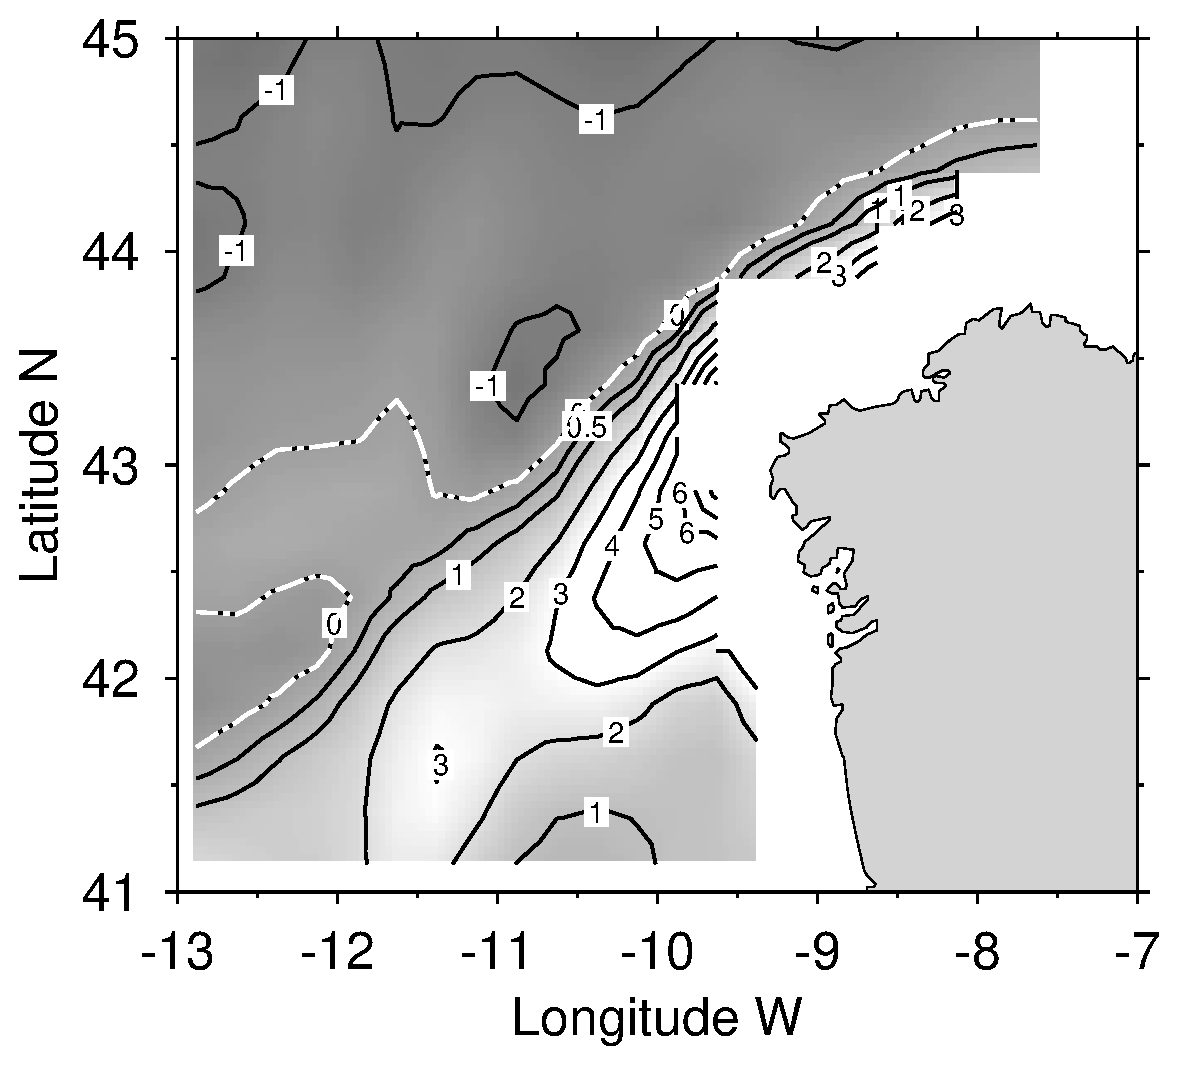
\includegraphics[height=8cm]{ekman_pum_1999723}%ekman_pum_1999723}
\caption{Vertical Ekman pumping velocities on 22 July 1999 in
m/day, positive upwards.} \label{fig:ekman}
\end{figure}

This maximum wind curl produces upwelling velocities given by
\(w=k\cdot(\nabla \times \frac{\tau}{f\rho} )\), where $k,\tau,f$
and $\rho$ are vertical unit vector, wind stress, Coriolis
parameter and density of water. This Ekman pumping is caused
solely by the divergent Ekman fluxes in the presence of spatially
variable wind and is unrelated to the coastal upwelling.  An
example is shown in Fig~\ref{fig:ekman} for measured winds on 22
July 1999 corresponding to a wind field similar to
Fig~\ref{fig:windsreconfig}a. Positive Ekman pumping velocities
indicative of upwelling can be seen south of the maximum wind curl
northern limit in Fig~\ref{fig:windseofseasonal}b and towards the
west coast. Maximum vertical velocities coincided with the axis of
maximum curl and decreased from 6\veld near Cape Finisterre to
1\veld farthest offshore. Calculations on a similar day in March
2000 yielded a similar pattern except vertical velocities were
smaller by a factor of 2 and decreased rapidly on the west coast.
The strong winds in June 1995 (Figs~\ref{fig:windsslp}a and b)
were again like the 1999 case. We conclude summer occurrences of
this wind pattern lead to upwelling velocities of 5-6\veld off
Cape Finisterre. These are smaller than the ones (up to 20\veld)
reported by \nocite{munchow00}\markcite{{\it M\"{u}nchow }[2000]}
off Point Conception, California. His finer sampling covered a
much smaller area which defined a maxima wind curl ridge 80km long
and 10km wide. In our case, the ridge extends 320km in length and
90km in width and vertical velocities are likely to reach higher
values nearer to the shore at Cape Finisterre.
\begin{figure}
\centering
\includegraphics[height=8cm]{wind_july9977march00320}
\caption{Example of measured winds from the offshore buoys on 7
July 1999 (black) and 20 March 2000 (red).} \label{fig:rev}
\end{figure}

\citet{Munchow00} reported flow separation in the wind field at
Point Conception in the presence of upwelling. He argued that the
lower sea surface temperatures enhanced the vertical stability of
the marine layer, which is capped by a temperature inversion.
Coastal upwelling can modify air temperatures by as much as
1-5\deg C over timescales of 12-24 hours \citep{Samelson02}. As in
\citet{Enriquez95}, the marine layer flow becomes supercritical
and separates from the coast causing the wind curl and Ekman
pumping velocities. We see some evidence of wind flow separation
in the lee of Cape Finisterre during the summer upwelling regime.
For example the buoy wind data for 7 July 1999 (Fig~\ref{fig:rev})
show measured north coast and Finisterre winds flowing nearly
opposite to west coast winds, suggestive of strong flow separation
at the cape. Similar north coast winds were common throughout
March 2000 and after 14 June 1999, but flow separation only
occurred in the presence of cold upwelled water around Cape
Finisterre during the 1999 examples. Hence, there are some
evidences that the PUNC strengthen both near the coast and after
the start of the coastal upwelling generating larger wind curl and
associated Ekman pumping velocities increasing shorewards. The
positive wind curl would cause a poleward alongshore pressure
gradient as indicated by model studies of \citet{Wang97}. However,
finer scale wind observations near Finisterre and atmospheric
observations would be needed to reach a definitive conclusion.

The existence of recurring wind curl west of Cape Finisterre will
influence the vertical water structure to cause doming of the
isopycnals. \citet{Munchow00} showed that a similar wind curl
influenced the vertical water structure to cause doming of the
isopycnals.  A similar local effect on the shelf circulation may
be expected around Cape Finisterre. The systematically weaker
southward velocities observed at the west coast buoy (S) compared
to the Finisterre buoy (F) are consistent with such a cyclonic
tendency but we presently have no hydrographic evidence to verify
it. Capes also have a significant impact on the alongshore
variability of the upwelling flow field
\citep{Crepon84,Dale01,Rosenfeld94}, producing nonlinear effects
accompanying the acceleration of the flow around the capes, and a
cyclonic tendency downstream. Doming could help explain the
persistence of the Finisterre filament following cessation of
favourable wind patterns, but again, observational evidence of the
detailed hydrographic and current structure near the cape is
lacking.


Winter winds in general showed larger variability than summer
winds during both a ``typical'' (2000-2001) and ''atypical''
(1999-2000) seasonal year. Downwelling wind patterns emerged from
CEOF analysis during both the 1999-2000 and winter 2001 analyses.
E,NE and N winds were predominant during both winters reaching
speeds in the range 15-20 \vel, higher than the 10-15 \vel range
of summer winds. However their persistence was far less (4-6 days)
than during summer ($\sim$12 days). Both winters saw the PUNC wind
field predominate during sustained periods in March and February
respectively. Its effect on the SST field was the disappearance on
the north coast, but not the west coast, of the warm temperature
anomaly indicative of poleward flow only.

It is difficult to define transitional regimes, non-upwelling to
upwelling and vice versa in terms of the wind forcing because of
the absence of any clear seasonal cycle.  Extension of the
analyses to a longer period will provide better information, but
it appears that as long as the meridional sea surface temperature
gradient is present, (nearly until July) upwelling winds do not
fully set up upwelling; even sustained winds provoking upwelling
early in the season do not develop filaments, e.g. April-May 2001.

\section{Conclusions}
Investigation of the QuikSCAT and in situ wind fields in the
Galician upwelling region around Cape Finisterre has shown:
\begin{itemize}
  \item    The wind field is far from homogeneous in the region so that
wind observations at a single point, coastal or offshore, will not
necessarily be representative of coastal conditions over any
significant distance.

  \item   The wind field's long-term mean summer and winter patterns are
not necessarily representative of particular years when, as we
have seen, summer-like patterns may dominate in winter also.

  \item   Similar Wind Modes were obtained in all CEOF analysis, of both
satellite derived and \emph{in situ} buoy measurements, and of
different length and seasonal period.

  \item   Summer time wind fields have a small number of dominant
patterns, discernible in complex empirical orthogonal analysis,
that are responsible for the typical distributions of upwelling in
and off the Galician coast.

  \item   One pattern produces north coast, but no west coast,
upwelling. In years when this pattern dominates, the Cape
Finisterre filament is strong but no others develop. The filament
is partly supplied by cold water from the north coast but also,
importantly, by local open ocean upwelling produced by the wind
stress curl, which extends in a maximum SW from the cape.

  \item   Another pattern produces west coast upwelling, but no
north coast upwelling.  When this pattern persists, west coast
filaments develop at favored locations other than Finisterre and
may extend up to 200km offshore.

  \item   These patterns may alternate producing brief episodes or north
or west coast upwelling with little filament development, or a
combined pattern may occur that produces weak upwelling on both
coasts with a localized maximum at Finisterre, where the wind lies
parallel to the coast.

  \item   Winter time wind patterns show strong similarities to those of
summer, symptomatic of frequent short occurrences of winter
upwelling during our study years.

  \item   The onset of the winter poleward flow regime as indicated by
presence of the warm water anomaly along the continental slope is
delayed after the cessation of summer upwelling winds.  Likewise
the spring onset of upwelling lags significantly the commencement
of favorable winds, though subsequent upwelling events respond
rapidly to wind changes.

  \item   North coast currents were more variable in all records
  and showed the largest velocities.
\end{itemize}
